\documentclass{beamer}
%Information to be included in the title page:
\title{Model Antrian \textit{Multi-Server:} M/M/c}
\subtitle{dengan Pengantar Model Stokastik dan Teori Antrian \\ dengan R dan QtsPlus}
\author{Bisma Rohpanca Joyosumarto (2106635581)}
\institute{Departemen Matematika FMIPA UI \\ Universitas Indonesia}
\date{
    Rabu, 13 November 2024

    Riset Operasi
    
    Tahun Ajaran 2024/2025 Semester Ganjil
}

% === bismastyle.sty ===
\AtBeginSection[]
{
  \begin{frame}{Daftar isi}
    \tableofcontents[currentsection]
  \end{frame}
}

\addtobeamertemplate{navigation symbols}{}{%
    \usebeamerfont{footline}%
    \usebeamercolor[fg]{footline}%
    \hspace{1em}%
    \insertframenumber/\inserttotalframenumber
}

\newcommand{\pars}[1]{\left(#1\right)}
\newcommand{\brackets}[1]{\left[#1\right]}
\newcommand{\braces}[1]{\left\{#1\right\}}

\usepackage{hyperref}
\usepackage{graphicx}
% === akhir bismastyle.sty ===

\begin{document}

\frame{\titlepage}

\begin{frame}{Table of Contents}
    \tableofcontents
\end{frame}

\section[Pengantar Model Stokastik dan Teori Antrian. dengan praktik di R]{Pengantar Model Stokastik dan Teori Antrian \\ dengan praktik di R}

\begin{frame}{Teori Antrian dan Model Stokastik}
    \begin{itemize}
        \item Dalam suatu \textbf{antrian \textit{(queue)}}, orang bisa masuk mengantri, dilayani, kemudian meninggalkan antrian
        \item Apabila ada beberapa pelayan, tiap baris/pelayan disebut \textit{server}, sehingga secara keseluruhan, terdapat satu antrian dengan sejumlah \textit{server}
        \item Pada dasarnya, proses mengantri bisa dimodel dengan melihat dua aspek: proses datangnya orang, dan proses perginya orang
        \item Di kuliah Pengantar Sains Data (Metode Statistika), kita sudah kenal \textbf{distribusi Poisson} yang memodelkan probabilitas banyaknya kemunculan dalam suatu satuan waktu, dalam yang namanya \textbf{proses Poisson}
        \item Baik datangnya orang maupun perginya orang, masing-masing bisa dimodelkan sebagai proses Poisson
    \end{itemize}
\end{frame}

\begin{frame}{Proses Poisson dan Rantai Markov}
    \begin{itemize}
        \item Sifat utama proses Poisson adalah \textbf{sifat Markov} atau \textbf{sifat \textit{memoryless:}} probabilitas kedatangan \textbf{tidak tergantung kapan datangnya}
        \item Proses Poisson adalah contoh \textbf{rantai Markov waktu kontinu} atau \textbf{\textit{continuous-time Markov chain} (CTMC)}
        \item CTMC itu sendiri adalah perumuman dari \textbf{rantai Markov waktu diskrit} atau \textbf{\textit{discrete-time Markov chain} (DTMC)}
    \end{itemize}
\end{frame}

\subsection{Rantai Markov Waktu Diskrit (DTMC)}

\begin{frame}{Definisi DTMC}
    Secara umum, dalam suatu rantai Markov, ada sejumlah "keadaan" atau \textit{state} yang terhitung (bisa berhingga), ada waktu, dan ada probabilitas berpindah dari satu \textit{state} ke \textit{state} lain.

    Suatu DTMC, misal \( \braces{X_t} \), terdiri dari
    \begin{itemize}
        \item Suatu \textit{state space} atau himpunan \textit{state} \( S \), berisi semua kemungkinan "keadaan" atau \textit{state}
        \item $X_t$ sebagai variabel acak untuk tiap \( t \), yang nilainya bisa berupa \textit{state} apa saja yang ada di \( S \). Sehingga, \( \braces{X_t} \) adalah barisan variabel acak
        \item Himpunan indeks waktu, biasanya \( T = \braces{0, 1, 2, \dots} \)
    \end{itemize}
    dan memenuhi \textbf{sifat Markov} atau \textbf{\textit{Markov property}} sebagai berikut:
    \begin{align*}
        \text{Pr}&\braces{X_{n+1} = j \, \mid \, X_0 = i_0, \, \dots \, X_{n-1} = i_{n-1}, X_n = i} \\
        &= \text{Pr}\braces{X_{n+1} = j \, \mid \, X_n = i}
    \end{align*}
    Artinya: probabilitas nilai \( X_t \) di waktu ke-\(\pars{n+1}\) hanya bergantung pada probabilitas di waktu ke-\(n\). Seolah-olah, tidak ada ingatan sama sekali tentang apa yang terjadi sebelum waktu ke-\(n\).

    %DTMC adalah contoh \textbf{proses stokastik \textit{(stochastic process)}}.
\end{frame}

\begin{frame}{DTMC stasioner}
    \begin{itemize}
        \item Kita bisa notasikan
        \[ P_{ij}^{n,n+1} = \text{Pr}\braces{X_{n+1} = j \, \mid \, X_n = i} \]
        yang disebut \textit{one-step transition probability}, dari \(X_n\) yang berada di \textit{state} \(i\) menjadi \(X_{n+1}\) yang berada di \textit{state} \(j\)
        \item Apabila nilai \(P_{ij}\) \textbf{tidak tergantung kapan}, maka rantai Markov disebut \textbf{stasioner}, dengan \textit{stationary transition probabilities}
        \item Dengan demikian, kita bisa menyusun \textbf{\textit{transition probability matrix} (TPM)} sebagai berikut, misalkan \(S=\braces{0,1,2,\dots}\):
        \[ P = \begin{pmatrix}
            P_{00} & P_{01} & P_{02} & \dots \\
            P_{10} & P_{11} & P_{12} & \dots \\
            \vdots & \vdots & \vdots & \ddots
        \end{pmatrix} \]
        dengan
        \[ P_{ij} = \text{Pr}\braces{X_{n+1} = j \, \mid \, X_n = i} \]
        sehingga baris ke-\(i\), kolom ke-\(j\) mengandung probabilitas transisi dari \textit{state} \(i\) ke \textit{state} \(j\).
    \end{itemize}
\end{frame}

\begin{frame}{Contoh DTMC: \textit{A Shoeshine Shop}}
    Misalkan ada usaha kecil oles sepatu. Hanya ada satu pelayan dan dua kursi pelanggan.
    \begin{itemize}
        \item Apabila kedua kursi kosong, orang cenderung tidak sadar bahwa itu adalah tempat oles sepatu, sehingga tidak datang.
        \item Namun, ketika salah satu kursi terisi, probabilitas kursi lainnya ikut terisi menjadi dua kali lipat dari biasanya.
        \item Ketika ada dua pelanggan, probabilitas satu pelanggan selesai adalah empat kali probabilitas keduanya belum selesai.
        \item Misalkan juga, tidak mungkin dua pelanggan datang sekaligus ataupun selesai sekaligus, dan tidak mungkin selesainya satu orang langsung diikuti datangnya pelanggan baru.
    \end{itemize}

    Ada empat keadaan yang mungkin, misalnya \( S = \braces{0,1,2,3} \) sebagai berikut
    \begin{enumerate}
        \item[(0)] Kedua kursi kosong
        \item[(1)] Kursi pertama saja diisi
        \item[(2)] Kursi kedua saja diisi
        \item[(3)] Kedua kursi diisi
    \end{enumerate}
\end{frame}

\begin{frame}{TPM untuk Contoh DTMC}
    TPM dari situasi di atas adalah seperti berikut:
    \[ P = \begin{pmatrix}
        0.5 & 0.25 & 0.25 & 0 \\
        0.25 & 0.25 & 0 & 0.5 \\
        0.25 & 0 & 0.25 & 0.5 \\
        0 & 0.4 & 0.4 & 0.2
    \end{pmatrix} \]
    Perhatikan bahwa sumasi tiap baris adalah satu. Ini akibat sifat probabilitas. Dari suatu \textit{state} \(i\), dia bisa ke \textit{state} lainnya (atau bahkan tetap di \textit{state} yang sama) dengan probabilitas masing-masing kemungkinan sesuai baris ke-\(i\).
\end{frame}

\begin{frame}{Diagram Transisi untuk Contoh DTMC}
    TPM bisa divisualisasikan sebagai \textbf{diagram transisi} atau \textbf{\textit{transition diagram}} sebagai berikut

    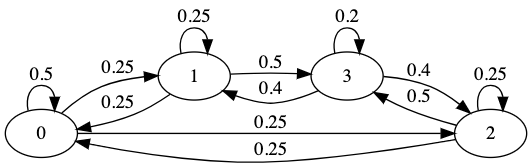
\includegraphics[scale=0.5]{gambar/fig01_dtmc.png}

    \begin{itemize}
        \item Tiap simpul melambangkan \textit{state}.
        \item Tiap busur dari \(i\) ke \(j\) melambangkan transisi, dengan label \(P_{ij}\)
    \end{itemize}
    \textit{Fun fact:} rantai Markov adalah versi probabilistik dari automata hingga.
\end{frame}

\begin{frame}{Simulasi dan Analisis DTMC di R}
    Gunakan \textit{package} markovchain
\end{frame}

\subsection{Proses Poisson}

\begin{frame}{Distribusi Poisson}
    \begin{itemize}
        \item Distribusi Poisson adalah distribusi diskrit yang memodelkan probabilitas untuk banyaknya kemunculan dalam suatu satuan waktu
        \item Hanya memliki satu parameter: rata-rata kemunculan per satuan waktu, biasa disebut \( \lambda \)
        \item Contoh: \( \text{Pois}(3) \), yaitu distribusi Poisson dengan rata-rata \( \lambda = 3 \)

        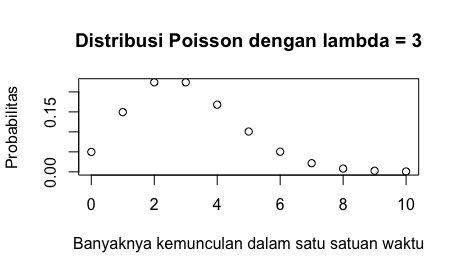
\includegraphics[scale=0.5]{gambar/fig02_dist_pois.png}
    \end{itemize}
\end{frame}

\begin{frame}{PMF untuk Distribusi Poisson}
    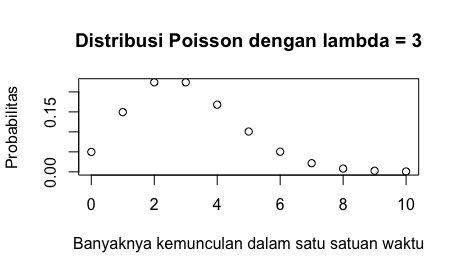
\includegraphics[scale=0.4]{gambar/fig02_dist_pois.png}

    Gambar di atas adalah contoh gambar PMF \textit{(probability mass function)} dari distribusi Poisson, yaitu nilai probabilitas untuk tepat \(x\) kemunculan dalam satu satuan waktu:
    \[ \text{Pr}(X=x) = \frac{e^{-\lambda} \lambda^x}{x} \]
    Contohnya, nilai PMF di \(x=2\) untuk \(\lambda = 3\) orang/menit adalah
    \[ \text{Pr}(X=2) = \frac{e^{-3} 3^2}{2} \approx 0.2240418 \]
    yaitu probabilitas datangnya \textbf{tepat dua} orang dalam satu menit.
\end{frame}

\begin{frame}{CDF untuk Distribusi Poisson}
    
\end{frame}

\subsection{Rantai Markov Waktu Kontinu (CTMC)}

\subsection{\textit{Birth-Death Process}}

\subsection{Antrian dan Notasinya}

\section{Antrian M/M/c}

\subsection{M/M/c secara umum}

\subsection{Kasus khusus: Antrian M/M/1}

\subsection{Simulasi M/M/c di R}

\subsection{M/M/c di QtsPlus}

\section{Lampiran: Tautan dan \textit{GitHub repository}}

\begin{frame}{Lampiran: Tautan dan \textit{GitHub repository}}
    Untuk \textit{package} R yang digunakan:
    \begin{itemize}
        \item markovchain: \url{https://github.com/spedygiorgio/markovchain}

        \item queuecomputer: \url{https://github.com/AnthonyEbert/queuecomputer}
        
        \item queueing: \url{https://cran.r-project.org/web/packages/queueing/index.html}
    \end{itemize}

    Tautan lainnya:

    \begin{itemize}
        \item QtsPlus v4.0: \url{https://mason.gmu.edu/~jshortle/fqt5th.html}
        
        \item \textit{GitHub repository} untuk presentasi ini (termasuk kode): \url{https://github.com/BismaBRJ/intro_stokastik_antrian_r_2024/}
    \end{itemize}
\end{frame}

\end{document}